\subsection{Indexing}
\subsubsection{Lý thuyết}
\begin{itemize}
    \item Khái niệm:
        \begin{itemize}
            \item Indexing là một cấu trúc dữ liệu phụ trợ giúp tăng tốc việc tìm kiếm và truy cập dữ liệu trong cơ sở dữ liệu.
            \item Chỉ mục thường được xây dựng trên một hoặc nhiều trường, cung cấp đường dẫn truy cập hiệu quả đến các bản ghi trong bảng dữ liệu.
        \end{itemize}
    \item Các loại chỉ mục phổ biến: 
        \begin{itemize}
            \item Dựa trên tệp được sắp xếp: Single-level Ordered Indexes.
            \item Dựa trên các cấu trúc dữ liệu cây: Multilevel indexes, B+-trees.
            \item Các loại chỉ mục khác:
                \begin{itemize}
                    \item Hash indexes.
                    \item Bitmap indexes.
                    \item Function-based indexes.
                \end{itemize}
        \end{itemize}
    \item Single-level Ordered Indexes. Bao gồm: 
        \begin{itemize}
            \item Primary Indexes: 
                \begin{itemize}
                    \item Đặc điểm:
                        \begin{itemize}
                            \item Được tạo trên khóa chính (primary key) của bảng.
                            \item Chỉ mục này sắp xếp dữ liệu trong bảng theo thứ tự của khóa chính.
                            \item Mỗi bản ghi trong bảng có một giá trị khóa chính duy nhất.
                        \end{itemize}
                    \item Cấu trúc: Thường là dense index hoặc sparse index.
                        \begin{itemize}
                            \item Dense Index: Có một mục nhập chỉ mục cho mỗi bản ghi trong bảng.
                            \item Sparse Index: Chỉ lưu chỉ mục cho một số bản ghi nhất định (chỉ mục thưa).
                        \end{itemize}
                \end{itemize}
            \item Clustering Indexes:
                \begin{itemize}
                    \item Đặc điểm:
                        \begin{itemize}
                            \item Sắp xếp dữ liệu vật lý trong bảng theo một hoặc nhiều cột, gọi là khóa cluster.
                            \item Không nhất thiết phải là khóa chính, nhưng thường là một khóa duy nhất.
                            \item Một bảng chỉ có thể có một cluster index.
                        \end{itemize}
                    \item Cấu trúc: Clustered Index tạo ra một mối liên kết giữa thứ tự vật lý của các bản ghi và giá trị của cột được sắp xếp.
                \end{itemize}
            \item Secondary Indexes:
                \begin{itemize}
                    \item Đặc điểm:
                        \begin{itemize}
                            \item Được tạo trên bất kỳ cột nào không phải khóa chính hoặc khóa cluster.
                            \item Dùng để hỗ trợ truy vấn nhanh trên các cột khác không sắp xếp vật lý trong bảng.
                            \item Một bảng có thể có nhiều secondary index.
                        \end{itemize}
                    \item Cấu trúc: Thường là dense index, vì mỗi giá trị trong cột cần có một mục nhập trong chỉ mục.
                \end{itemize}
        \end{itemize}
\end{itemize}

\subsubsection{Indexing trong PostgreSQL}
\indent PostgreSQL hỗ trợ nhiều loại chỉ mục: 
\begin{itemize}
    \item B-Tree: Chỉ mục mặc định, phù hợp với truy vấn so sánh (=, <, >, BETWEEN).
        \begin{itemize}
            \item Cách khởi tạo:
\begin{lstlisting}[language=SQL]
CREATE INDEX idx_btree ON employees (age);
\end{lstlisting}
            \item Cách sử dụng:
\begin{lstlisting}[language=SQL]
SELECT * FROM employees WHERE age > 30;
\end{lstlisting}
        \end{itemize}
    \item Hash Index: Hash index được sử dụng chủ yếu cho các phép so sánh bằng (=). Tuy nhiên, nó ít được sử dụng hơn so với B-tree vì không hỗ trợ các phép so sánh khác như <, >.
        \begin{itemize}
            \item Cách khởi tạo:
\begin{lstlisting}[language=SQL]
CREATE INDEX idx_hash ON employees USING HASH (name);
\end{lstlisting}
            \item Cách sử dụng:
\begin{lstlisting}[language=SQL]
SELECT * FROM employees WHERE name = 'ABC';
\end{lstlisting}
        \end{itemize}
    \item GiST (Generalized Search Tree) là loại chỉ mục linh hoạt, cho phép chỉ mục trên các kiểu dữ liệu phức tạp như range, point, circle, text search, và hỗ trợ các toán tử: ($<<$,    \&<,   \&>,   $>>$,   $<<$|,   \&<|,   |\&>,   |$>>$,   @>,   <@,   $~=$,   \&\&).
        \begin{itemize}
            \item Cách khởi tạo:
\begin{lstlisting}[language=SQL]
CREATE INDEX idx_gist ON locations USING GiST (location);
\end{lstlisting}
            \item Cách sử dụng:
\begin{lstlisting}[language=SQL]
SELECT * FROM locations WHERE location @> 'POINT(1 1)';
\end{lstlisting}
        \end{itemize}
    \item SP-GiST (Space-partitioned Generalized Search Tree) là một loại chỉ mục hỗ trợ dữ liệu không gian và có thể sử dụng cho các loại dữ liệu như point, circle, và các loại dữ liệu không gian khác ($<<$,   $>>$,   $~$=,    <@,   $<<$|,   |$>>$).
        \begin{itemize}
            \item Cách khởi tạo:
\begin{lstlisting}[language=SQL]
CREATE INDEX idx_spgist ON locations USING SPGIST (location);
\end{lstlisting}
            \item Cách sử dụng:
\begin{lstlisting}[language=SQL]
SELECT * FROM locations WHERE location <-> 'POINT(1 1)' < 0.5;
\end{lstlisting}
        \end{itemize}
    \item GIN (Generalized Inverted Index) chủ yếu được sử dụng với các kiểu dữ liệu như array, jsonb, và tsvector. (<@,   @>,   $=$,   \&\&).
        \begin{itemize}
            \item Cách khởi tạo:
\begin{lstlisting}[language=SQL]
CREATE INDEX idx_gin ON documents USING GIN (content);
\end{lstlisting}
            \item Cách sử dụng:
\begin{lstlisting}[language=SQL]
SELECT * FROM documents WHERE content @@ to_tsquery('search_term');
\end{lstlisting}
        \end{itemize}
    \item BRIN (Block Range INdex)) thích hợp với các bảng rất lớn có dữ liệu theo thứ tự. BRIN không tạo chỉ mục cho từng giá trị mà tạo chỉ mục cho các block dữ liệu ($<,   <=,   =,   >=,   >\&$).
        \begin{itemize}
            \item Cách khởi tạo:
\begin{lstlisting}[language=SQL]
CREATE INDEX idx_brin ON measurements USING BRIN (timestamp);
\end{lstlisting}
            \item Cách sử dụng:
\begin{lstlisting}[language=SQL]
SELECT * FROM measurements WHERE timestamp > '2024-01-01';
\end{lstlisting}
        \end{itemize}
\end{itemize}
 
\subsubsection{Indexing trong MongoDB}
\indent MongoDB, với kiến trúc phi quan hệ, hỗ trợ các loại chỉ mục:
\begin{itemize}
    \item Single Field Index: Index trên một trường duy nhất. Đây là loại chỉ mục đơn giản và phổ biến nhất.
    \begin{figure}[H]
        \centering
        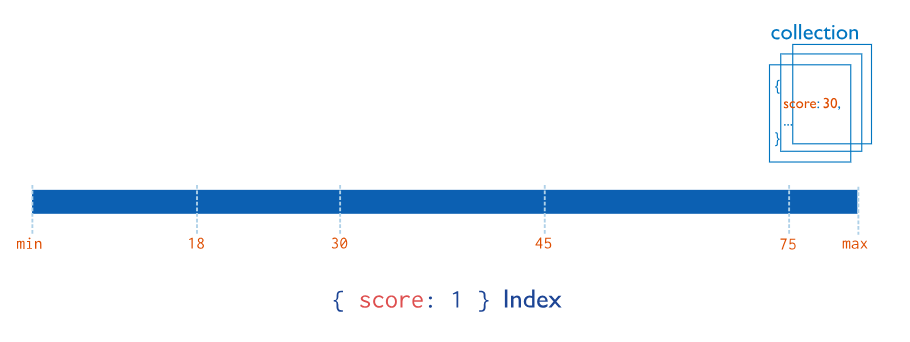
\includegraphics[width=\textwidth]{Image/2.2.3a.png}
        \caption{Single Field Index}
    \end{figure}
        \begin{itemize}
            \item Cách khởi tạo:
\begin{lstlisting}[language=SQL]
db.collection.createIndex({ fieldName: 1 }); 
\end{lstlisting}
            \item Cách sử dụng:
\begin{lstlisting}[language=inform]
db.users.createIndex({ age: 1 });
db.users.find({ age: { $gt: 25 } });
\end{lstlisting}
        \end{itemize}
    \item Compound Index: Index trên nhiều trường, phù hợp khi các truy vấn lọc dựa trên nhiều trường
    \begin{figure}[H]
        \centering
        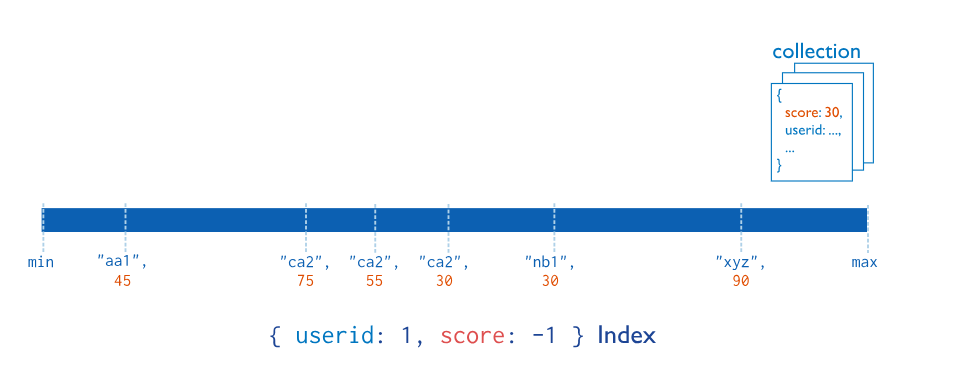
\includegraphics[width=\textwidth]{Image/2.2.3b.png}
        \caption{Compound Index}
    \end{figure}
        \begin{itemize}
            \item Cách khởi tạo:
\begin{lstlisting}[language=inform]
db.collection.createIndex({ field1: 1, field2: -1 });
\end{lstlisting}
            \item Cách sử dụng:
\begin{lstlisting}[language=inform]
db.users.createIndex({ age: 1, city: -1 });
db.users.find({ age: { $gte: 30 }, city: "New York" });
\end{lstlisting}
        \end{itemize}
    \item Multikey Index: Dành cho các trường chứa mảng. Mỗi giá trị trong mảng sẽ được lập chỉ mục.
    \begin{figure}[H]
        \centering
        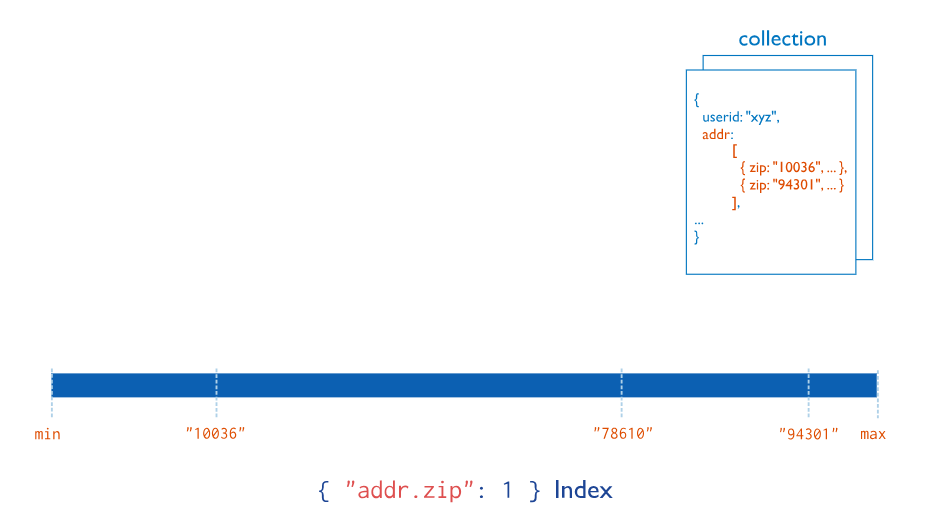
\includegraphics[width=\textwidth]{Image/2.2.3c.png}
        \caption{Multikey Index}
    \end{figure}
        \begin{itemize}
            \item Cách khởi tạo:
\begin{lstlisting}[language=inform]
db.collection.createIndex({ fieldName: 1 });
\end{lstlisting}
            \item Cách sử dụng:
\begin{lstlisting}[language=SQL]
db.products.createIndex({ tags: 1 });
db.products.find({ tags: "electronics" });
\end{lstlisting}
        \end{itemize}
    \item Geospatial Index: Dành cho dữ liệu không gian địa lý như tọa độ 2D hoặc 2DSphere.
        \begin{itemize}
            \item Cách khởi tạo:
\begin{lstlisting}[language=inform]
db.collection.createIndex({ location: "2dsphere" });
\end{lstlisting}
            \item Cách sử dụng:
\begin{lstlisting}[language=inform]
db.places.createIndex({ location: "2dsphere" });
db.places.find({
location: {
$near: {
$geometry: { type: "Point", coordinates: [40.7128, -74.0060] },
$maxDistance: 1000
}
}
});
\end{lstlisting}
        \end{itemize}
    \item  Wildcard Index: Index trên tất cả các trường hoặc một tập con trường, phù hợp với dữ liệu không có cấu trúc.
        \begin{itemize}
            \item Cách khởi tạo:
\begin{lstlisting}
db.collection.createIndex({ "$**": 1 });
\end{lstlisting}
            \item Cách sử dụng:
\begin{lstlisting}[language=inform]
db.logs.createIndex({ "$**": 1 });
db.logs.find({ "details.ip": "192.168.1.1" });
\end{lstlisting}
        \end{itemize}
    \item Hashed Index: Lập chỉ mục dựa trên giá trị băm của một trường, thường dùng để cân bằng tải truy vấn.
        \begin{itemize}
            \item Cách khởi tạo:
\begin{lstlisting}[language=SQL]
db.collection.createIndex({ fieldName: "hashed" });
\end{lstlisting}
            \item Cách sử dụng:
\begin{lstlisting}[language=SQL]
db.users.createIndex({ user_id: "hashed" });
db.users.find({ user_id: 12345 });
\end{lstlisting}
        \end{itemize}
\end{itemize}


\subsubsection{So sánh và kết luận}
\begin{itemize}
    \item Đa dạng loại index: PostgreSQL hỗ trợ nhiều loại index phức tạp hơn phù hợp cho các truy vấn phức tạp và dữ liệu quan hệ, trong khi MongoDB tập trung vào các loại index phù hợp với dữ liệu không cấu trúc và dễ thay đổi.
    \item Ứng dụng và tối ưu hóa: PostgreSQL thường được sử dụng trong các ứng dụng đòi hỏi tính toàn vẹn, với các chỉ mục như GiST và GIN. Ngược lại, MongoDB phù hợp với các ứng dụng yêu cầu tốc độ và tính linh hoạt cao, với các chỉ mục như Multi-key và Geospatial.
    \item  Cấu trúc dữ liệu: PostgreSQL sử dụng các loại index để tối ưu hóa dữ liệu quan hệ, trong khi MongoDB sử dụng các loại index để tối ưu hóa dữ liệu tài liệu và các kiểu dữ liệu phi cấu trúc khác.
\end{itemize}
\begin{table}[H]
    \centering
    \begin{tabular}{|L{3.2cm}|L{5cm}|L{5cm}|} \hline 
         \textbf{Tiêu chí so sánh }&  \textbf{PostgreSQL}&  \textbf{MongoDB}\\ \hline 
         Sự tương thích &  Hỗ trợ nhiều toán tử, phép toán, thích hợp cho các truy vấn dữ liệu quan hệ phức tạp & Tập trung vào các loại index phù hợp với dữ liệu không cấu trúc và dễ thay đổi.\\ \hline 
         Ứng dụng và tối ưu hóa &  Đòi hỏi tính toàn vẹn của dữ liệu. & Thích hợp với dữ liệu thường xuyên thay đổi, tính linh hoạt cao, yêu cầu tốc độ truy xuất nhanh.\\ \hline 
         Cấu trúc dữ liệu &  Tối ưu hóa dữ liệu quan hệ. &  Tối ưu hóa dữ liệu tài liệu.\\ \hline
    \end{tabular}
    \caption{So sánh về Indexing giữa PostgreSQL và MongoDB}
    \label{tab:indexing}
\end{table}
\indent \textbf{Kết luận:}

\newpage





